
%%%%%%%%%%%%%%%%                                ~~~~~~~~~~~~~~~~~~~~~~~~~~~~~~~~~~~~~~~~~~~~~~~~~~
% CONDITIONALS %
%%%%%%%%%%%%%%%%                                ~~~~~~~~~~~~~~~~~~~~~~~~~~~~~~~~~~~~~~~~~~~~~~~~~~

\newif\ifPeerReview\PeerReviewfalse             % Whether to create the PeerReview version or
                                                % Journal version
\newif\ifFlatArchive\FlatArchivefalse           % Whether archive is flat (messy) or contain 
                                                % subfolders for graphics etc.
\newif\ifFloatAtEnd\FloatAtEndfalse             % Available in PeerReview mode:
                                                % Place floats at end of document?
\newif\ifTODO\TODOtrue                          % Use todo notes?

%%%%%%%%%%%%%%                                  ~~~~~~~~~~~~~~~~~~~~~~~~~~~~~~~~~~~~~~~~~~~~~~~~~~
% ECUA style %
%%%%%%%%%%%%%%                                  ~~~~~~~~~~~~~~~~~~~~~~~~~~~~~~~~~~~~~~~~~~~~~~~~~~

\documentclass[10pt,a4paper]{article}
\usepackage{template/ecua}

%%%%%%%%%%%%%%%%%%%%%%%%%%%%%%                  ~~~~~~~~~~~~~~~~~~~~~~~~~~~~~~~~~~~~~~~~~~~~~~~~~~
% ECUA ''APPROVED'' PACKAGES %
%%%%%%%%%%%%%%%%%%%%%%%%%%%%%%                  ~~~~~~~~~~~~~~~~~~~~~~~~~~~~~~~~~~~~~~~~~~~~~~~~~~

% load some other useful packages
\usepackage{cite} % improved formatting for citation lists
\usepackage{graphicx}

%%%%%%%%%%%%%%%%%%%%%%%                         ~~~~~~~~~~~~~~~~~~~~~~~~~~~~~~~~~~~~~~~~~~~~~~~~~~
% ADDITIONAL PACKAGES %       
%%%%%%%%%%%%%%%%%%%%%%%                         ~~~~~~~~~~~~~~~~~~~~~~~~~~~~~~~~~~~~~~~~~~~~~~~~~~

\usepackage[table,dvipsnames,svgnames]{xcolor}
\newcounter{todoidx}

\ifTODO
   \definecolor{todobackground}{rgb}{0.95,0.95,0.95}
   \setlength\marginparsep{1pt}
   \setlength\marginparwidth{35pt}
   \newlength\marginparwidthsmall
   \setlength\marginparwidthsmall{\marginparwidth}
   \addtolength\marginparwidthsmall{-7pt}
   \newcommand\todo[1]{%
      \addtocounter{todoidx}{1}%
      {\color{Red}\fbox{\bf\thetodoidx{}}}%
      \marginpar{%
         {\vspace*{-10pt}\color{Red}\fbox{\bf\thetodoidx{}}}\\%
         \fcolorbox{red}{todobackground}{\parbox{\marginparwidthsmall}{\scriptsize #1}}}}

   \newcommand\todopar[1]{\fcolorbox{red}{white}{\parbox{0.97\linewidth}{#1}}}
\else
%    \usepackage[disable]{./todonotes} 
   \newcommand\todo[1]{}
\fi

\newenvironment{narrow}[2]{%
\begin{list}{}{%
\setlength{\topsep}{0pt}%
\setlength{\leftmargin}{#1}%
\setlength{\rightmargin}{#2}%
\setlength{\listparindent}{\parindent}%
\setlength{\itemindent}{\parindent}%
\setlength{\parsep}{\parskip}}%
\item[]}{\end{list}}

\usepackage{float}

%%%%%%%%%%                                      ~~~~~~~~~~~~~~~~~~~~~~~~~~~~~~~~~~~~~~~~~~~~~~~~~~
% MACROS %       
%%%%%%%%%%                                      ~~~~~~~~~~~~~~~~~~~~~~~~~~~~~~~~~~~~~~~~~~~~~~~~~~


\newcommand\Grey[1]{{\color{Grey}#1}}
\newcommand\Red[1]{{\color{Red}#1}}
\newcommand\Blue[1]{{\color{Blue}#1}}
\newcommand\DarkBlue[1]{{\color{DarkBlue}#1}}
\newcommand\LightBlue[1]{{\color{LightBlue}#1}}
\newcommand\Brown[1]{{\color{Brown}#1}}
\newcommand\Green[1]{{\color{Green}#1}}
\newcommand\SeaGreen[1]{{\color{SeaGreen}#1}}
\newcommand\Yellow[1]{{\color{yellow}#1}}
\newcommand\Orange[1]{{\color{orange}#1}}

\newcommand\nn{\nonumber\\}

\newcommand\nmat[1]{\begin{matrix}#1\end{matrix}}
\newcommand\bmat[1]{\begin{bmatrix}#1\end{bmatrix}}
\newcommand\case[1]{\begin{cases}#1\end{cases}}
\newcommand\textbox[2]{\footnotesize\text{\parbox{#1}{\centering\emph{#2}}}}

\newcommand\rand{\text{rand}}
\newcommand\randn{\text{randn}}
\newcommand\rect{\text{rect}}
\newcommand\sinc{\text{sinc}}
\newcommand\tr{\text{tr}}
\newcommand\adj{\text{adj}}

% \newcommand\max{\text{max}}
\newcommand\argmin{\text{argmin}}

\newcommand\qqquad{\quad\qquad}
\newcommand\qqqquad{\qquad\qquad}

\renewcommand\l[1]{\left#1}
\renewcommand\r[1]{\right#1}

% {\text{\parbox{1.5cm}{\centering volume hyper- sphere}}}

%Keyword colouring:
\newcommand\kw[1]{#1}
\newcommand\parm[1]{#1}%\color{Black}#1\color{Black}}

\newcommand\of[1]{\scriptstyle(\parm{#1})\displaystyle}
\newcommand\df[1]{\scriptstyle[\parm{#1}]\displaystyle}
\newcommand\var[3]{#1_\text{#2}\of{#3}}

\newcommand\diag{\text{diag}}

% \raisebox{lift}[extend-above-baseline][extend-below-baseline]{text}
\newcommand\mt[1]{\text{\emph{#1}}} %mt = mathtext
\newcommand\mathnorm{\textstyle}
\newcommand\mathbig[1]{\displaystyle#1\mathnorm}
\newcommand\mathsmall[1]{\scriptstyle#1\mathnorm}
\newcommand\mathtiny[1]{\scriptscriptstyle#1\mathnorm}
\newcommand\sfrac[2]{\scriptstyle\raisebox{0.25pt}[0pt][0pt]{$\frac{#1}{#2}$}\mathnorm}
\newcommand\nfrac[2]{\textstyle\frac{#1}{#2}\displaystyle}

\newcommand\sumu[1]{\sum\limits^{#1}\,}
\newcommand\suml[1]{\sum\limits_{#1}\,}
\newcommand\sumb[2]{\sum\limits_{#1}^{#2}\,}

\newcommand\produ[1]{\prod\limits^{#1}\,}
\newcommand\prodl[1]{\prod\limits_{#1}\,}
\newcommand\prodb[2]{\prod\limits_{#1}^{#2}\,}

%Math macros:
\newcommand\diff[2]{\frac{\kw{d}\,\textstyle #1\scriptstyle}{\kw{d\parm{#2}}}\displaystyle}
\newcommand\ddiff[2]{\frac{\kw{d^2}\,\displaystyle #1\scriptstyle}{\kw{d\parm{#2}}^2}\displaystyle}

\renewcommand\d[1]{\scriptstyle\kw{\,d\parm{#1}}\displaystyle}

% These commands are mutually exclusive. Remember to "renew" in v2.
\newcommand\intb[4]{\int\limits_{#3}^{#4} #1 \d{#2}} % \int{exp}{var}{from}{to}
\newcommand\intl[3]{\int\limits_{#3} #1 \d{#2}} % \int{exp}{var}{for all}
\newcommand\intu[2]{\int #1 \d{#2}} % \int{exp}{var}{for all}

\newcommand\T{^{\scriptscriptstyle T}}
\renewcommand\H{^{\scriptscriptstyle H}}

\renewcommand\vec[1]{\boldsymbol{#1}}
\newcommand\mat[1]{\boldsymbol{#1}}


\renewcommand*\a{\vec a}
\renewcommand*\i{\vec i}
\renewcommand*\k{\vec k}
\newcommand*\n{\vec n}
\newcommand*\p{\vec p}
\newcommand*\s{\vec s}
\newcommand*\w{\vec w}
\newcommand*\x{\vec x}
\newcommand*\y{\vec y}

\newcommand*\A{\mat A}
\newcommand*\B{\mat B}
\newcommand*\C{\mat C}
\newcommand*\E{\mat E}
% \renewcommand*\H{\mat H}
\renewcommand*\P{\mat P}
\newcommand*\eP{\mat{\hat P}}
\newcommand*\R{\mat R}
\newcommand*\Ri{\R^{-1}}
\newcommand*\eR{\mat{\hat R}}
\newcommand*\eRi{\hat{\mat R}\,\!^{-1}}
\newcommand*\Navg{N_\text{avg}}
\newcommand*\W{\mat W}
\newcommand*\X{\mat X}
\newcommand*\Xd{\X_{\!\Delta}}
\newcommand*\Y{\mat Y}

\renewcommand*\L{\mat \Lambda}
\newcommand*\U{\mat U}
% \renewcommand*\t{\mathtiny{^T}}
% \newcommand*\h{\mathtiny{^H}}
\renewcommand*\t{^T}
\newcommand*\h{^H}

\newcommand\D{\vec\nabla} %Del: Vector differential operator - nabla
\newcommand\Dx{\vec\nabla\times}
\newcommand\Dd{\vec\nabla\cdot}

\usepackage{tikz}
\usetikzlibrary{shapes,snakes}
\usepackage{amsmath,amssymb}

\newenvironment{outline}
{\begin{itemize}}
{\end{itemize}}

%    \definecolor{todobackground}{rgb}{0.95,0.95,0.95}
%    \setlength\marginparsep{3pt}
%    \setlength\marginparwidth{42pt}
%    \newlength\marginparwidthsmall
%    \setlength\marginparwidthsmall{\marginparwidth}
%    \addtolength\marginparwidthsmall{-7pt}
%    \newcommand\todo[1]{%
%       \addtocounter{todoidx}{1}%
%       {\color{Red}\fbox{\bf\thetodoidx{}}}%
%       \marginpar{%
%          {\vspace*{-10pt}\color{Red}\fbox{\bf\thetodoidx{}}}\\%
%          \fcolorbox{red}{todobackground}{\parbox{\marginparwidthsmall}{#1}}}}
% 

% correct bad hyphenation here
% \hyphenation{op-tical net-works semi-conduc-tor}


%%%%%%%%%%%%%%%%%%                              ~~~~~~~~~~~~~~~~~~~~~~~~~~~~~~~~~~~~~~~~~~~~~~~~~~
% DOCUMENT START %
%%%%%%%%%%%%%%%%%%                              ~~~~~~~~~~~~~~~~~~~~~~~~~~~~~~~~~~~~~~~~~~~~~~~~~~

\title{A GPU Implementation of Capon for an Active Sonar System}

\author{%
\begin{tabular}{p{30mm}p{125mm}}
Jo~Inge~Buskenes & Department of Informatics, University of Oslo, Norway \\
Jon~Petter~Aasen & Department of Informatics, University of Oslo, Norway \\
Carl-Inge~Colombo~Nilsen & Department of Informatics, University of Oslo, Norway \\
\end{tabular}
}

\begin{document}

\maketitle

\section{Introduction}

When forming images from an active sonar system employing a phased array, the lateral \gls{SNR} and resolution will largely depend on the choice of weights applied to each of the array channels. 
The Capon beamformer has been around for quite som time now. It is adaptive 

Delays and weights are applied to each of the sensor channels to ensure that signals emanating from a pixel of interest add constructively, while noise and interference from other regions add destructively. This method of adjusting the spatial focus of the antenna is commonly referred to as a beamformer. A

Beamformer algorithms are distinction 

The Minimum Variance One of the most well established adaptive 

One of the main issues with adaptive beamformers is their computational complexity, and .

Most modern active sonar imaging systems record and process the incoming wavefield through the use of phased arrays. A pixel value in the image is estimated by digitally steering the arrays response to the corresponding region in space. This concept is called beamforming and involves applying a suitable set of delays and weights to each of the sensor channels to cause constrictive interference of the signals coming from the region of interest, and destructive interference of anything else. Ideally, we want a spatial response 

If a beamformer only employ a static set of weights and delays, it is referred to as a conventional one. Applying , which  Various weight sets, or windows, may be added, Adaptive beamformers, on the other hand, attempts to find an optimal spatial response that best fits the incoming wavefield.  The most common approach is perform a rough adjustment using a static set of delays, and compute a new set of weights at each time instant. 



\todopar{Case:
\begin{itemize}
\item JOE
\item Sonar. Channel count up to 32/64 ish channels?
\item Other articles evaluates Capon image quality, and some have shown that speedups can be achieved by reducing the complexity of the traditional Capon algorithm or by implementing specific versions on a GPU.
\item This article compare a few promising ways to implement Capon in general, in light of general complexity and suitability for implementation on a CPU and GPU.
\end{itemize}
}

\begin{itemize}
\item As briefly as possible, introduce beamforming.
\item Adaptive beamformer's potential lies in its ability to suppress interference power
\item Why adaptive beamformers struggle in active sonar systems. Correlated noise, robustification kills the adaptive potential. Quite computationally intensive. Constraints must be applied in one way or another - parameters must be tuned.
\item The three main ways to implement Capon \cite{Capon1969} is \todo{not entirely true?}
\begin{itemize}
\item Traditional way: Build $\eR$ and solve $\w = \frac{\Ri\a}{\a\H\Ri\a}$. 
\item Iterative methods: Woodbury, Conjugated gradients
\item Beamspace
\item LCA (or other methods, as reference)
\end{itemize}
\item Choice of robustification parameters $L,M,\Delta$ largely impacts what the ``optimal'' way of implementing Capon 
\item In most imaging applications 
Outline:
\begin{itemize}
\item Speeding up: Build $\eR$ and solve $\w = \frac{\Ri\a}{\a\H\Ri\a}$. 
\item Iterative methods: Woodbury (Sherman Morrison), Conjugated gradients - show performance of GPU performance.
\item Woodbury: Must take the average over many samples in space and time - lots of (small) outerproducts. Can be used if not a lot of averaging is required.
\item Beamspace
\item LCA (or other methods, as reference)
\end{itemize}
\end{itemize}


\section{Methods}

\begin{align}
z[n] = \sumb{m=0}{M-1} w_m[n]^*x_m[n-\Delta_m] = \w\H[n]\Xd[n]
\end{align}
where
\begin{align}
\w[n] = \bmat{w_0[n]\\w_1[n]\\\vdots\\w_{M-1}[n]} \quad \text{and} \quad\Xd[n] = \bmat{x_0[n]\\x_1[n]\\\vdots\\x_{M-1}[n]}.
\end{align}

Minimum variance distortionless resonse \cite{Capon1969}
\begin{align}
\underset{\w[n]}{\argmin}\, E\{ |z[n]|^2 \} = \underset{\w[n]}{\argmin}\, \w\H[n]\R[n]\w[n], 
\end{align}
subject to
\begin{align}
\w\H[n]\a = 1,
\end{align}
where
\begin{align}
\R[n] = E\{ \x\x\H \}.
\end{align}
If $\eR$ is the estimate of $\R$, the solution to the MVDR beamformer is
\begin{gather*}
\vec w[n] = \frac{\hat{\mat R}\,\!^{-1}[n]\vec a}{\vec a\H\hat{\mat R}\,\!^{-1}[n]\vec a} = \frac{\text{\raisebox{1.9pt}{$\vec\chi$}}[n]}{\vec a\H\text{\raisebox{1.9pt}{$\vec\chi$}}[n]}
\end{gather*}
A robust estimate of $\eR$ is found by
\begin{itemize}
\item Spatial averaging to decorrelate noise from signal. \emph{Subarray averaging} used here.
\item Temporal averaging to ensure valid speckle statistics.
\item \emph{Diagonal loading} to ensure  numerical stability prior to inversion.
\item Choice of robustification parameters \cite{Synnevag2007}
\end{itemize}

Here $\vec a$ is a \emph{steering vector} that if set to $\vec 1$ steers towards broadside, and $\hat{\mat R}$ is an estimate of the spatial covariance matrix, often computed as
\begin{gather*}
r_{ij}[n] = \frac{1}{K(2N_{\text{avg}}+1)}\sumb{k=0}{K-1} \sumb{n'=n-N_{\text{avg}}}{n+N_{\text{avg}}} x_{i+k}[n']\,x_{j+k}[n'],
\end{gather*}
where $r_{ij}$ is the $(i,j)$'th element of the covariance matrix, $K$ is the number of subarrays, $2N_{\text{avg}}+1$ is the number of samples to perform time averaging over, and $\vec x_i[n']$ is the data recorded by the $i$'th sensor at sample $n'$. 

\emph{Diagonal loading} chosen as \cite{Synnevag2007}
\begin{align}
\varepsilon = \Delta \cdot \tr\{\eR[n]\}
\end{align}

\subsection{Traditional approach}

Let us first consider the \emph{computation of $\hat{\mat R}$}. Notice that when implementing the formula directly a lot of summations and multiplications will be repeated unnecessary. To illustrate this, consider for instance a case with $M=6$ sensors that are grouped into subarrays of length $L=3$ where all but one element overlap. Let us further assume that we need to average over 7 time samples, i.e. that $N_{\text{avg}} = 3$. 

These procedures are commutative, so the order in which we perform them does not matter. But for the sake of this example let us start by performing the time averaging. Assuming that $\vec x_i$ and $\vec x_j$ have a zero mean, a time averaged covariance coefficient $r_{ij}$ in $\hat{\mat R}$ may be obtained by (omitting the normalisation):
\begin{align*}
r_{ij}[n] &= \sumb{n'=n-N_{\text{avg}}}{n+N_{\text{avg}}} x_i[n']\,x_j[n'],
\end{align*}
which can be easily rewritten in a sliding window fashion
\begin{align*}
r_{ij}[n] &= r_{ij}[n-1] - x_i[n\text{-}N_\text{avg}\text{-}1]\,x_j[n\text{-}N_\text{avg}\text{-}1]
                         + x_i[n\text{+}N_\text{avg}]\,x_j[n\text{+}N_\text{avg}].
\end{align*}
Hence, whenever $N_\text{avg}>1$ the sliding window approach will demand less instructions at the expense of a slightly higher memory consumption. The next thing to realise is that not all $r_{ij}[n]$ need to be computed. Since $r_{ji} = r^*_{ij}$, and the subarrays only span $L$ elements, we only compute an upper triangular band of R (marked \Green{green})
\begin{figure}[H]
% \begin{narrow}{-3.5cm}{-3.5cm}
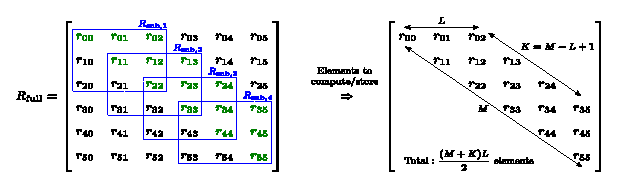
\includegraphics[width=\linewidth]{gfx/capon_build_R_full.eps}
\caption{Building $\hat{\mat R}$: Symmetry and element coverage}\label{buildingRfull}
% \end{narrow}
\end{figure}
The final step is to average all the subarray matrices to form $\hat{\mat R}$ by 
{\renewcommand*{\arraystretch}{1.8}
\begin{align*}
\hat{\mat R}_\text{sub} &= {\color{Blue}\mat R_{\text{sub},1} + \mat R_{\text{sub},2} + \mat R_{\text{sub},3} + \mat R_{\text{sub},4}} \\
&= \left[\;
\begin{matrix}
\color{Green}r_{00}+r_{11}+r_{22} & \color{Red}r_{01}+r_{12}+r_{23} & r_{02}+r_{13}+r_{24} \\
                                       & \color{Green}r_{11}+r_{22}+r_{33} & \color{Red}r_{12}+r_{23}+r_{34} \\
                                       &                                        & \color{Green}r_{22}+r_{33}+r_{44}
\end{matrix}
\;\right]
\end{align*}}%
Note that consecutive elements along the diagonals overlap on all but one covariance coefficient, hence a sliding window may also be used here. The subarray size $L$ is usually quite a bit larger than the time averaging window, so there is more to gain from implementing the sliding window here.\\\\

{\bf Method complexity:}\\
\begin{tabular}{l l}
No optimizations            & $2M^2\,(2\Navg+1)$ \\
Banded symmetric            & $L(2M-L+1)\,(2\Navg+1)$ \\
Sliding, banded, symmetric  & $1.5L(2M-L+1)$ \\
\end{tabular}\\\\



% \subsubsection{Computing $\text{\raisebox{1.9pt}{$\vec\chi$}} = \hat{\mat R}\,\!^{-1}\vec a$}

There are two ways of finding $\text{\raisebox{1.9pt}{$\vec\chi$}} = \hat{\mat R}\,\!^{-1}\vec a$, either by solving the equation directly or by inverting $\hat{\mat R}$ first. Solving the equation is less computationally intensive than inverting $\hat{\mat R}$, and seems like the obvious choice. However, with iterative methods for updating $\eRi$ for each range pixel the situation is changed...


\subsection{Iterative methods}

\begin{itemize}
\item Woodbury
\item Conjugated gradients
\end{itemize}


\subsection{Beamspace}

\begin{itemize}
\item Some minimum of background, and good references.
\end{itemize}


\section{Results/Discussion}


\begin{itemize}
\item Compare computational complexity vs. memory constraints for the various methods. Supporting plots.
\item Relate this to whether the favourable architecture is a CPU or a GPU \todo{check ``when to gpu article''}
\item Run benchmarks on some sonar dataset(s)
\end{itemize}


\section{Conclusion}

\begin{itemize}
\item When to use what.
\end{itemize}


% \ \\
% \IEEEPARstart{T}{o} form images from a modern phased array sonar system the received wavefield is usually recorded, and then postprocessed by a digital beamformer. The beamformer applies delays and weights to the sensor channels, the beamformer adjusts the arrays spatial response to focus at one pixel at a time.  such that signals emanating from regions of interest add constructively, while ensuring that noise and interference from other angles do not. 
% 
% The imaging capabilities of a modern phased array sonar system depend on physical attributes such element response and array geometry, the transmitted signal, as well as the beamforming method being used on transmission and reception. Beamforming is the concept of applying delays and weights to the sensors channels to steer the arrays response to points of interest. 

% 
% 
% Outline:
% \begin{itemize}
% \item Capon's resonse when applying robustification
% \item Choice of window functions makes little difference.
% \item Steering and mainlobewidths have outer bounds.
% \item Beamspace?
% \item Chosen window plots - what may they tell us? Variance intensity values when using various windows.
% \item Assymmetric windows?
% \end{itemize}
% 
% 
% \begin{align}
% z[n] = \sumb{m=0}{M-1} w_m[n]^*x_m[n-\Delta_m] = \w\H[n]\x[n-\Delta_m]
% \end{align}
% 
% 
% \section{Methods}
% 
% Basically, we are working with a practical implementation of the Capon beamformer that computes a set of weights $\vec w$ for every single sample $n$ by solving:
% \begin{gather*}
% \vec w[n] = \frac{\hat{\mat R}\,\!^{-1}[n]\vec a}{\vec a\H\hat{\mat R}\,\!^{-1}[n]\vec a} = \frac{\text{\raisebox{1.9pt}{$\vec\chi$}}[n]}{\vec a\H\text{\raisebox{1.9pt}{$\vec\chi$}}[n]}
% \end{gather*}%
% where
% % \newcommand\X{\text{\raisebox{2pt}{$\vec\chi$}}}
% \begin{gather*}
% \text{\raisebox{1.9pt}{$\vec\chi$}} = \hat{\mat R}\,\!^{-1}\vec a \qquad\qquad\text{is the solution to}\qquad\qquad \hat{\mat R}\text{\raisebox{1.9pt}{$\vec\chi$}} = \vec a.
% \end{gather*}

% 
% , and maximum suppression of while ensuring that the beamformer digitally  before each of the pixels are estimated one at a time. The resolution and contrast of such a system will depend on the systems spatial response, which ideally should be narrow  be very sharp in the desired direction its ability to achieve  fundamental principle of forming a sonar image is to record the received wavefield, 
% 
% image quality of a phased array sonar imaging systems depend on  the choice of weights to apply to each of the sensors are crucial. 
% 
% A modern phased array imaging system may be thought of as a spatial filter. To achieve the best possible performance, the 
% 
% resolution and contrast 
% 
% Adaptive beamformers have only recently been introduced in active sonar imaging. For a while they were considered unsuited for this purpose because the backscattered signal is largely correlated with the 
% 
% 
% 

%\begin{figure}[!t]
%\centering
%\includegraphics[width=2.5in]{myfigure}
% where an .eps filename suffix will be assumed under latex, 
% and a .pdf suffix will be assumed for pdflatex; or what has been declared
% via \DeclareGraphicsExtensions.
%\caption{Simulation Results}
%\label{fig_sim}
%\end{figure}


% An example of a double column floating figure using two subfigures.
% (The subfig.sty package must be loaded for this to work.)
% The subfigure \label commands are set within each subfloat command, the
% \label for the overall figure must come after \caption.
% \hfil must be used as a separator to get equal spacing.
% The subfigure.sty package works much the same way, except \subfigure is
% used instead of \subfloat.
%
% \begin{figure*}[!t]
% \centerline{\subfloat[Case I]\includegraphics[width=2.5in]{subfigcase1}%
% \label{fig_first_case}}
% \hfil
% \subfloat[Case II]{\includegraphics[width=2.5in]{subfigcase2}%
% \label{fig_second_case}}}
% \caption{Simulation results}
% \label{fig_sim}
% \end{figure*}
%
% Note that often IEEE papers with subfigures do not employ subfigure
% captions (using the optional argument to \subfloat), but instead will
% reference/describe all of them (a), (b), etc., within the main caption.


% An example of a floating table. Note that, for IEEE style tables, the 
% \caption command should come BEFORE the table. Table text will default to
% \footnotesize as IEEE normally uses this smaller font for tables.
% The \label must come after \caption as always.
%
%\begin{table}[!t]
%% increase table row spacing, adjust to taste
%\renewcommand{\arraystretch}{1.3}
% if using array.sty, it might be a good idea to tweak the value of
% \extrarowheight as needed to properly center the text within the cells
%\caption{An Example of a Table}
%\label{table_example}
%\centering
%% Some packages, such as MDW tools, offer better commands for making tables
%% than the plain LaTeX2e tabular which is used here.
%\begin{tabular}{|c||c|}
%\hline
%One & Two\\
%\hline
%Three & Four\\
%\hline
%\end{tabular}
%\end{table}


% Note that IEEE does not put floats in the very first column - or typically
% anywhere on the first page for that matter. Also, in-text middle ("here")
% positioning is not used. Most IEEE journals use top floats exclusively.
% However, Computer Society journals sometimes do use bottom floats - bear
% this in mind when choosing appropriate optional arguments for the
% figure/table environments.
% Note that, LaTeX2e, unlike IEEE journals, places footnotes above bottom
% floats. This can be corrected via the \fnbelowfloat command of the
% stfloats package.



\section{Conclusion}
The conclusion goes here.





% if have a single appendix:
%\appendix[Proof of the Zonklar Equations]
% or
%\appendix  % for no appendix heading
% do not use \section anymore after \appendix, only \section*
% is possibly needed

% use appendices with more than one appendix
% then use \section to start each appendix
% you must declare a \section before using any
% \subsection or using \label (\appendices by itself
% starts a section numbered zero.)
%

%%%%%%%%%%%%%%%%%%                              ~~~~~~~~~~~~~~~~~~~~~~~~~~~~~~~~~~~~~~~~~~~~~~~~~~
% DOCUMENT APPENDICES %
%%%%%%%%%%%%%%%%%%                              ~~~~~~~~~~~~~~~~~~~~~~~~~~~~~~~~~~~~~~~~~~~~~~~~~~


\section*{Acknowledgments}

The authors would like to thank...


\bibliographystyle{./ecua}
\bibliography{../../Library/library}


\end{document}


